\documentclass[]{article}
\usepackage{lmodern}
\usepackage{amssymb,amsmath}
\usepackage{ifxetex,ifluatex}
\usepackage{fixltx2e} % provides \textsubscript
\ifnum 0\ifxetex 1\fi\ifluatex 1\fi=0 % if pdftex
  \usepackage[T1]{fontenc}
  \usepackage[utf8]{inputenc}
\else % if luatex or xelatex
  \ifxetex
    \usepackage{mathspec}
  \else
    \usepackage{fontspec}
  \fi
  \defaultfontfeatures{Ligatures=TeX,Scale=MatchLowercase}
\fi
% use upquote if available, for straight quotes in verbatim environments
\IfFileExists{upquote.sty}{\usepackage{upquote}}{}
% use microtype if available
\IfFileExists{microtype.sty}{%
\usepackage{microtype}
\UseMicrotypeSet[protrusion]{basicmath} % disable protrusion for tt fonts
}{}
\usepackage[margin=1in]{geometry}
\usepackage{hyperref}
\hypersetup{unicode=true,
            pdftitle={Insurance dataset variables},
            pdfauthor={Rhian Davies},
            pdfborder={0 0 0},
            breaklinks=true}
\urlstyle{same}  % don't use monospace font for urls
\usepackage{graphicx,grffile}
\makeatletter
\def\maxwidth{\ifdim\Gin@nat@width>\linewidth\linewidth\else\Gin@nat@width\fi}
\def\maxheight{\ifdim\Gin@nat@height>\textheight\textheight\else\Gin@nat@height\fi}
\makeatother
% Scale images if necessary, so that they will not overflow the page
% margins by default, and it is still possible to overwrite the defaults
% using explicit options in \includegraphics[width, height, ...]{}
\setkeys{Gin}{width=\maxwidth,height=\maxheight,keepaspectratio}
\IfFileExists{parskip.sty}{%
\usepackage{parskip}
}{% else
\setlength{\parindent}{0pt}
\setlength{\parskip}{6pt plus 2pt minus 1pt}
}
\setlength{\emergencystretch}{3em}  % prevent overfull lines
\providecommand{\tightlist}{%
  \setlength{\itemsep}{0pt}\setlength{\parskip}{0pt}}
\setcounter{secnumdepth}{0}
% Redefines (sub)paragraphs to behave more like sections
\ifx\paragraph\undefined\else
\let\oldparagraph\paragraph
\renewcommand{\paragraph}[1]{\oldparagraph{#1}\mbox{}}
\fi
\ifx\subparagraph\undefined\else
\let\oldsubparagraph\subparagraph
\renewcommand{\subparagraph}[1]{\oldsubparagraph{#1}\mbox{}}
\fi

%%% Use protect on footnotes to avoid problems with footnotes in titles
\let\rmarkdownfootnote\footnote%
\def\footnote{\protect\rmarkdownfootnote}

%%% Change title format to be more compact
\usepackage{titling}

% Create subtitle command for use in maketitle
\newcommand{\subtitle}[1]{
  \posttitle{
    \begin{center}\large#1\end{center}
    }
}

\setlength{\droptitle}{-2em}
  \title{Insurance dataset variables}
  \pretitle{\vspace{\droptitle}\centering\huge}
  \posttitle{\par}
  \author{Rhian Davies}
  \preauthor{\centering\large\emph}
  \postauthor{\par}
  \date{}
  \predate{}\postdate{}


\begin{document}
\maketitle

\paragraph{Menu}\label{menu}

\begin{itemize}
\tightlist
\item
  \href{../ReadMe.html}{Read me}
\item
  \href{variables_description.html}{Variable descriptions}.
\item
  \href{Pairwise_correlations_for_value_B.html}{Pairwise correlation
  plots}.
\item
  \href{Chunking_CC.html}{Chunking CC}.
\item
  \href{Simple_offline_algorithms.html}{Simple offline clustering}
\end{itemize}

Data has 465115 rows. There are 10 features: Day, Time, Age of Driver,
Age of Car, Expected Value of Car, CC, Duration and Values A, B and C.
Lets consider them in turn.

\subsubsection{Day}\label{day}

\begin{itemize}
\tightlist
\item
  Values between 1 and 7
\item
  Assume they relate to day of week (1 = Sunday?)
\item
  Starts on a 6 and finishes on a 3 (Friday - Tuesday?)
\item
  There are \textasciitilde{}13 weeks of data \textasciitilde{} 3 months
\item
  I assume the data is collected continously
\item
  Any seasonality issues? Would need start date
\item
  Noticible difference in volume over weekday/weekends
\end{itemize}

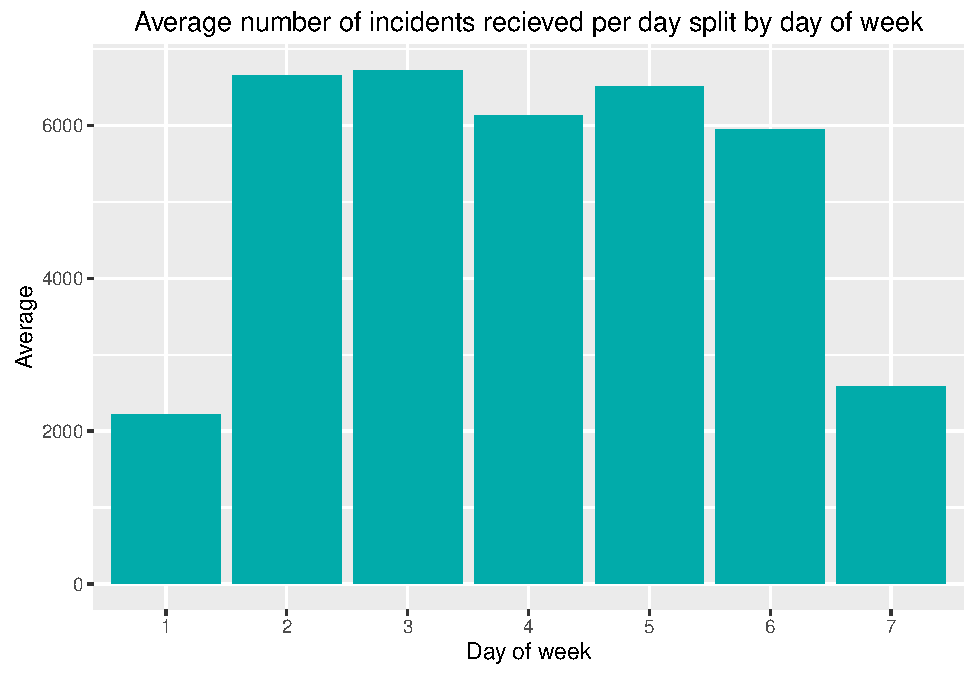
\includegraphics{variables_description_files/figure-latex/observations_per_day-1.pdf}

\subsubsection{Time}\label{time}

We can look at the distribution of requests across the full dataset.

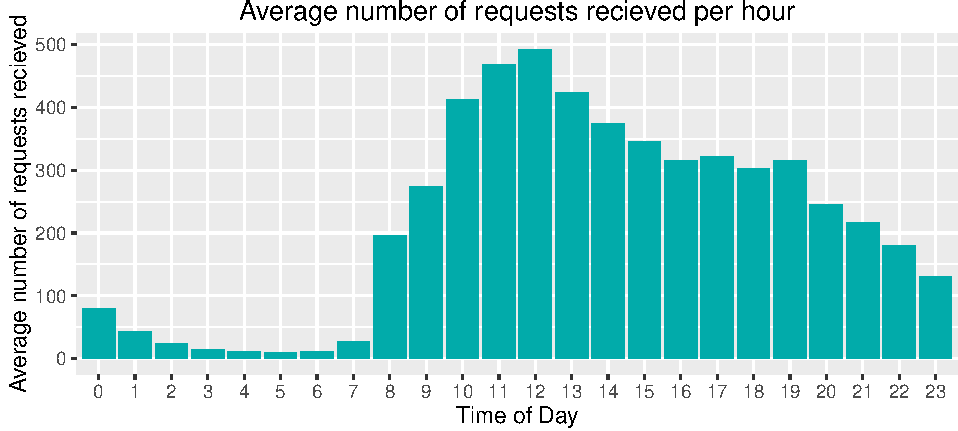
\includegraphics{variables_description_files/figure-latex/distribution_of_requests-1.pdf}

This is what we would expect to see - peak incidences beteen 10 and 6pm.

We can split the daily total requests by policy duration

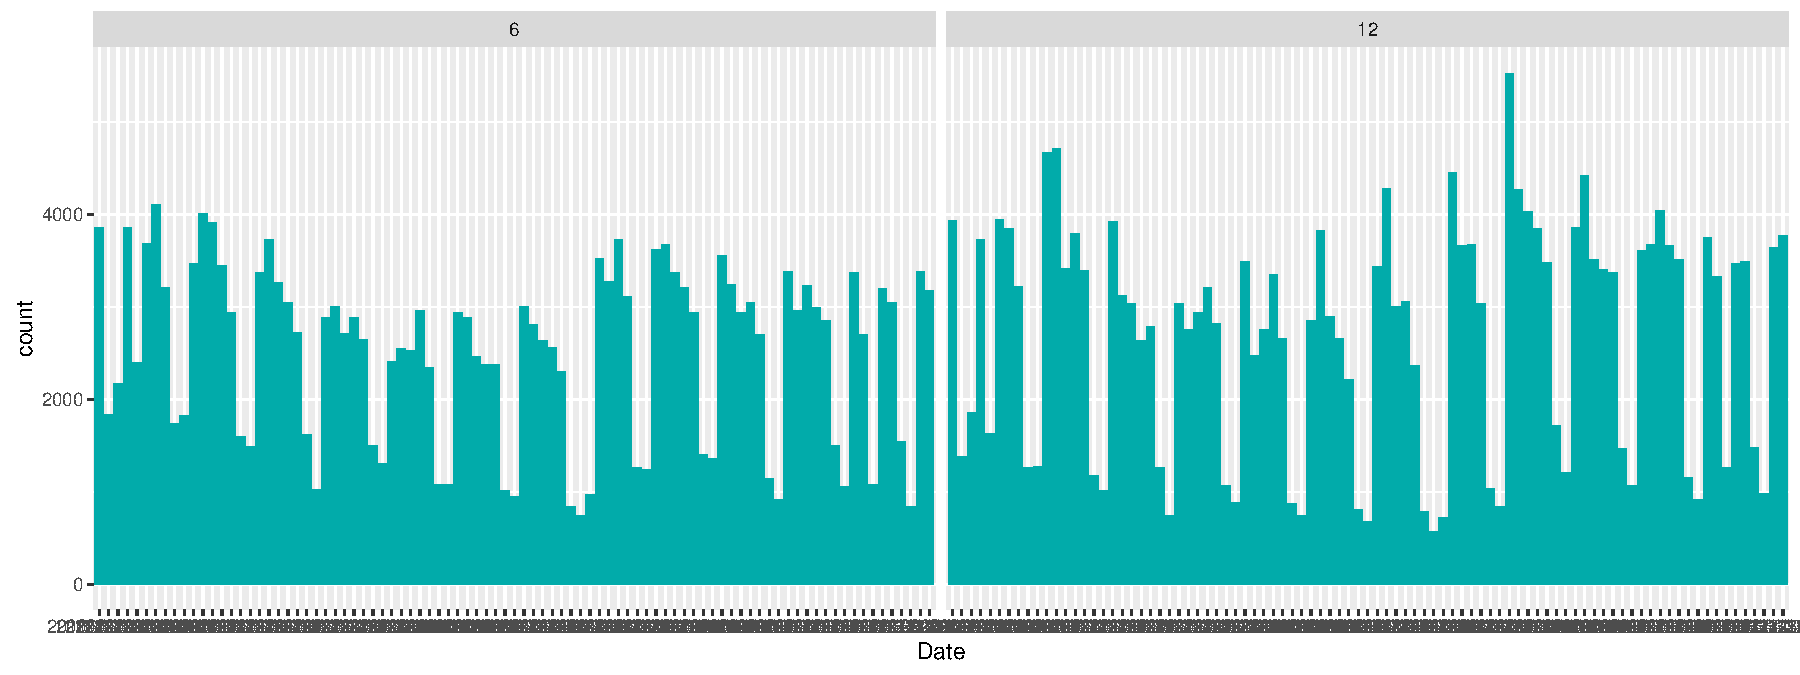
\includegraphics{variables_description_files/figure-latex/total_requests_policy_duration-1.pdf}

As above but summed by week (Friday - Thursday)
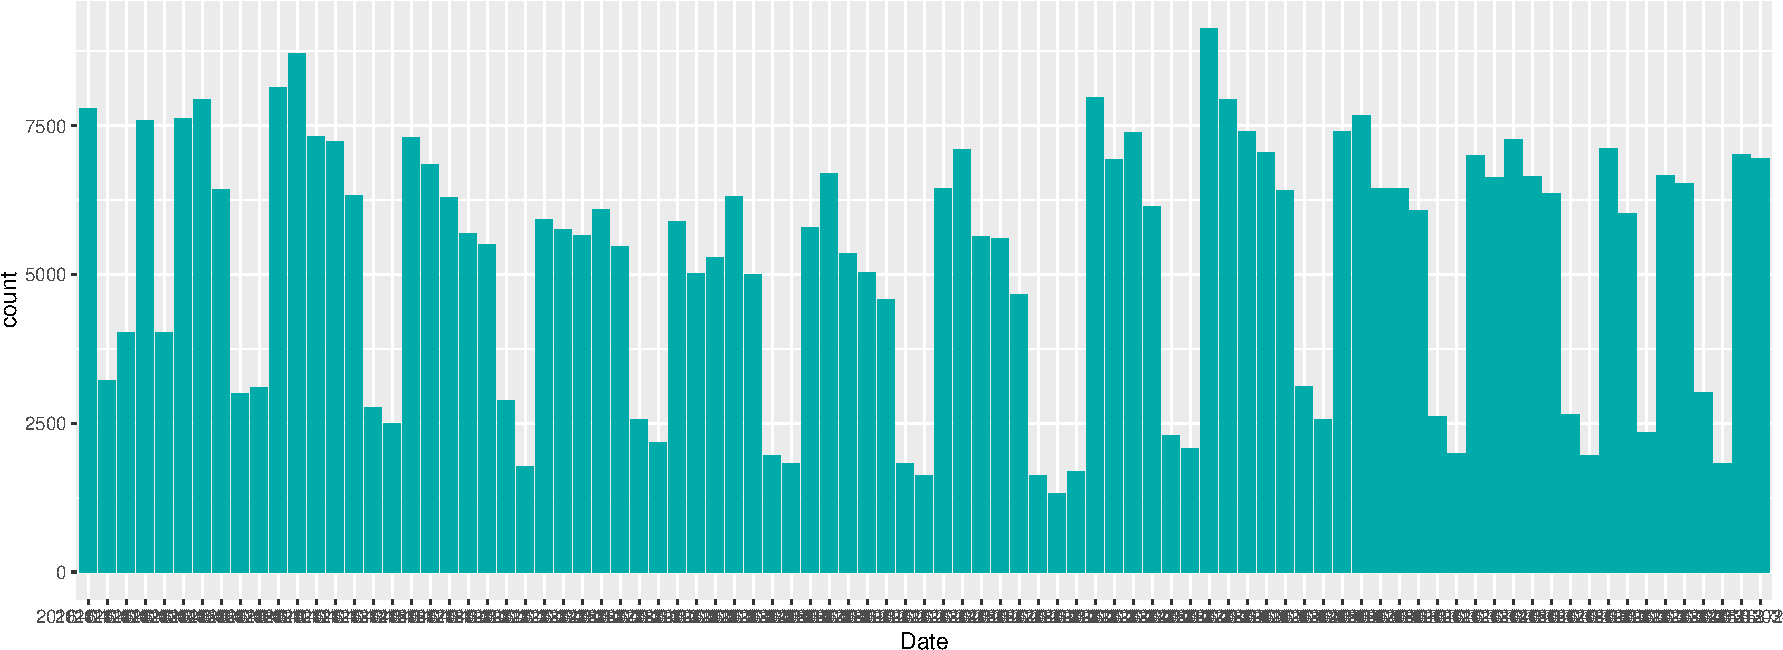
\includegraphics{variables_description_files/figure-latex/total_requests_policy_duration_week-1.pdf}

\begin{itemize}
\tightlist
\item
  Would like to know start date of collection
\item
  Some unusually low Mondays (bank holidays?)
\item
  Weeks 4-8 seem low, with a peak in week 9 - summer holidays?
\end{itemize}

We can also break down into time over all the days.

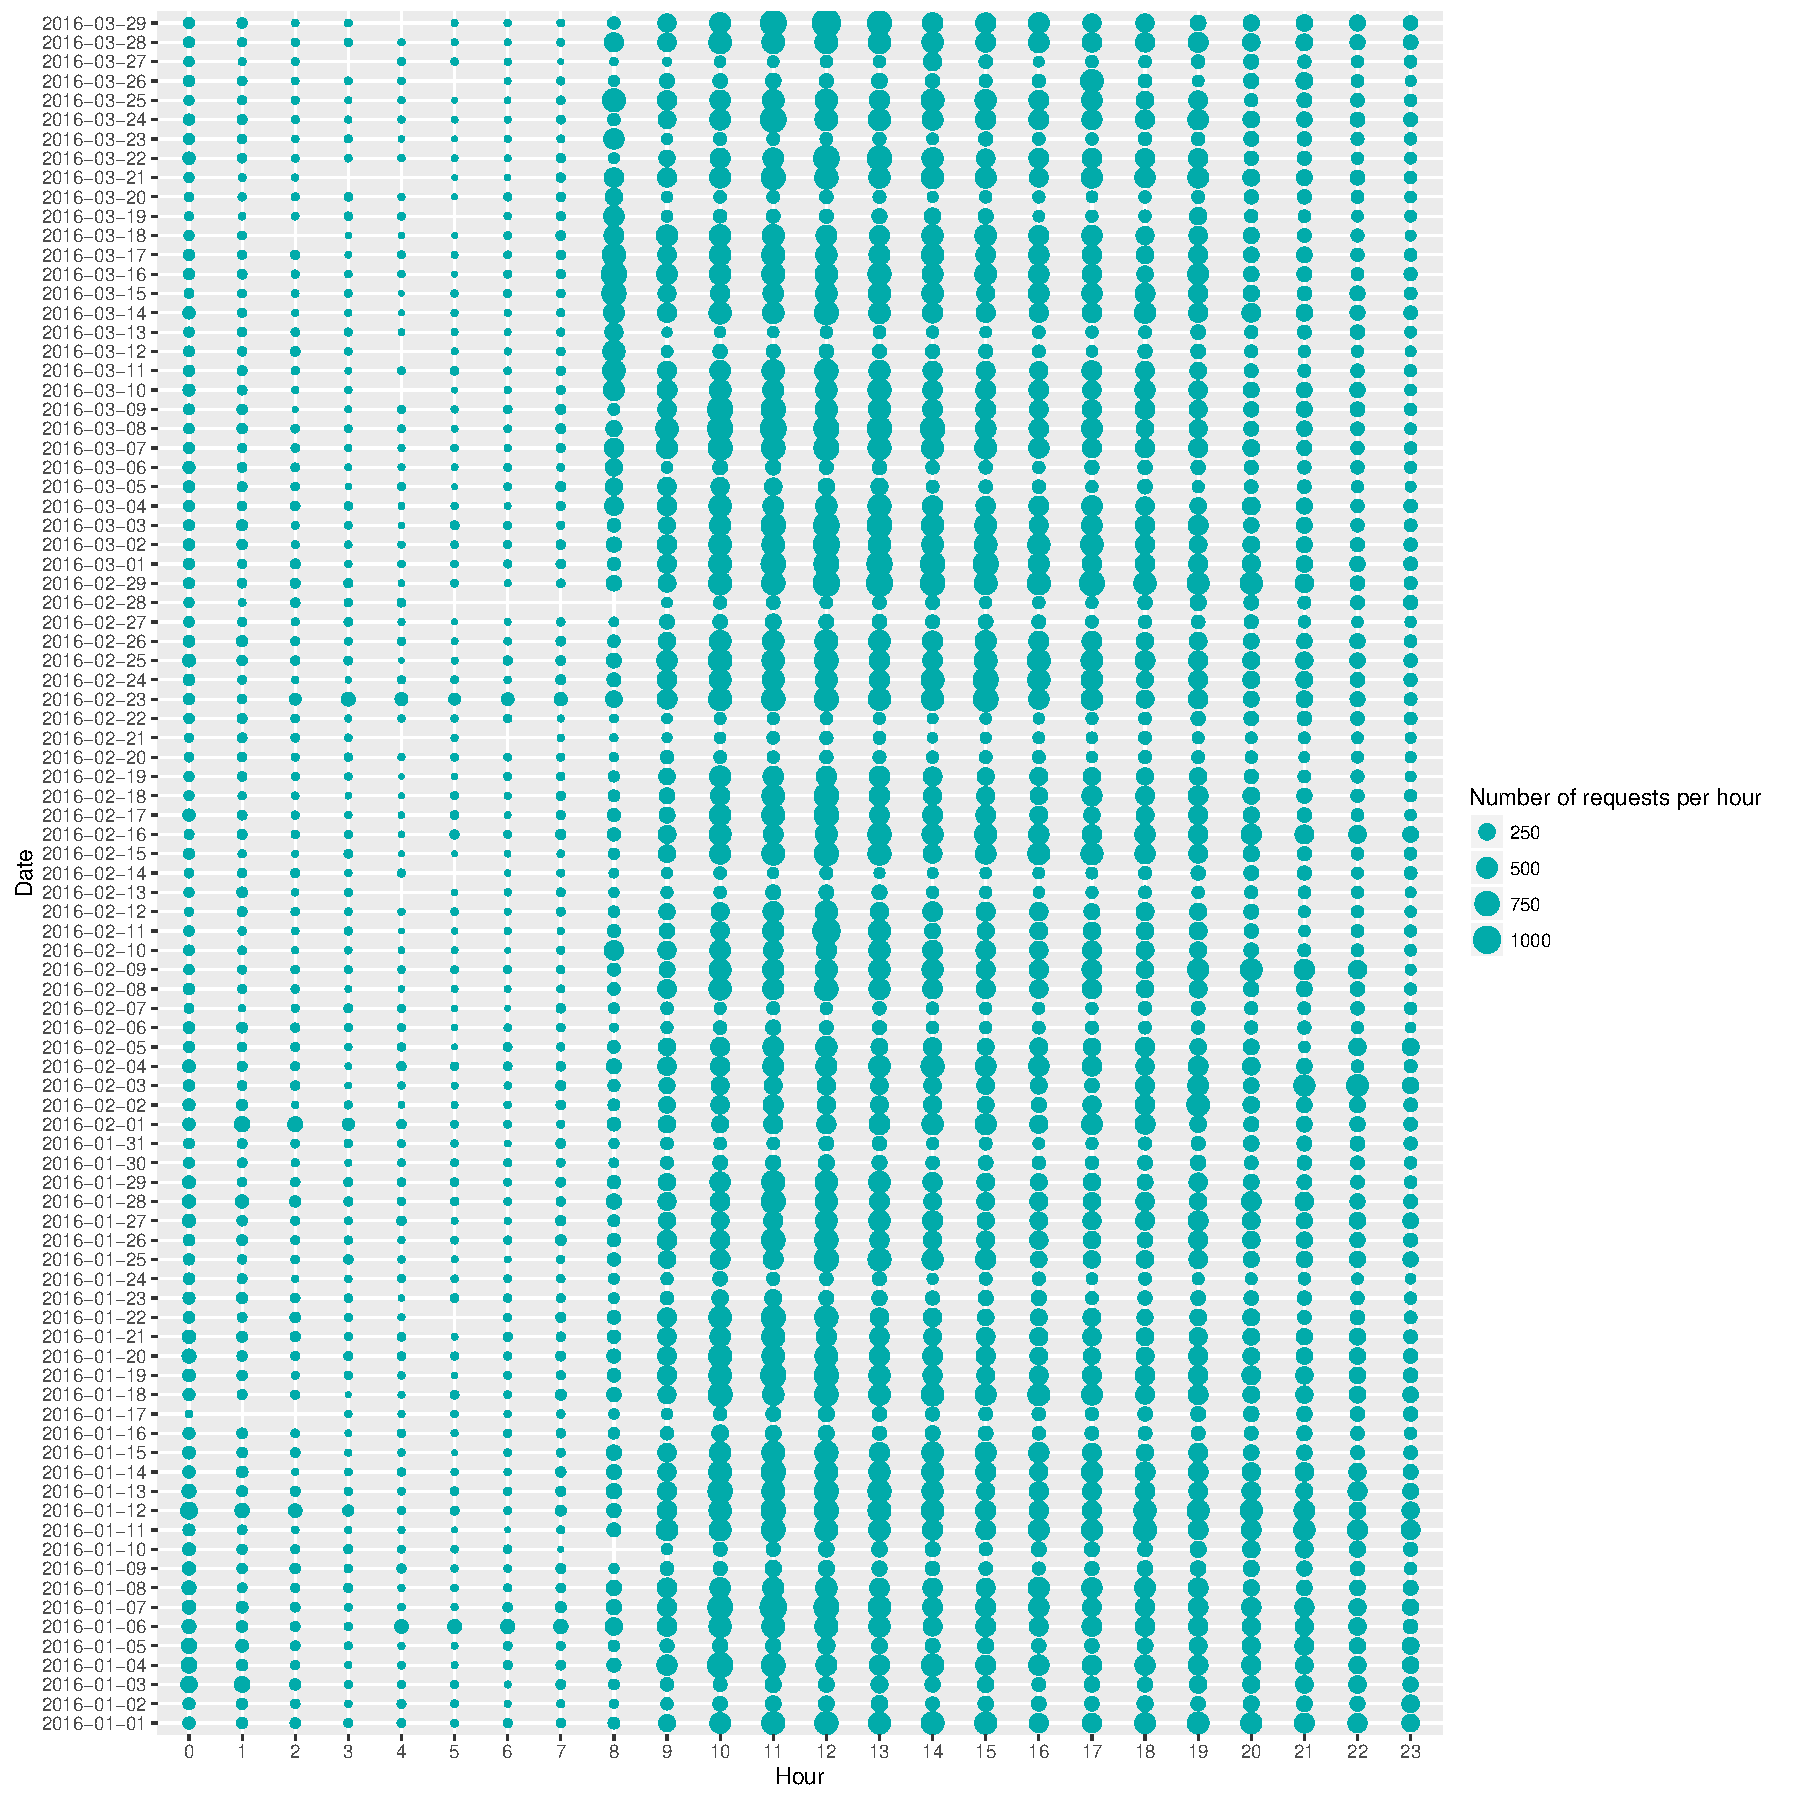
\includegraphics{variables_description_files/figure-latex/requests_per_hour-1.pdf}

\subsubsection{Age of Driver}\label{age-of-driver}

Age distribution is shown below - pretty standard ranging from 18 to 81.

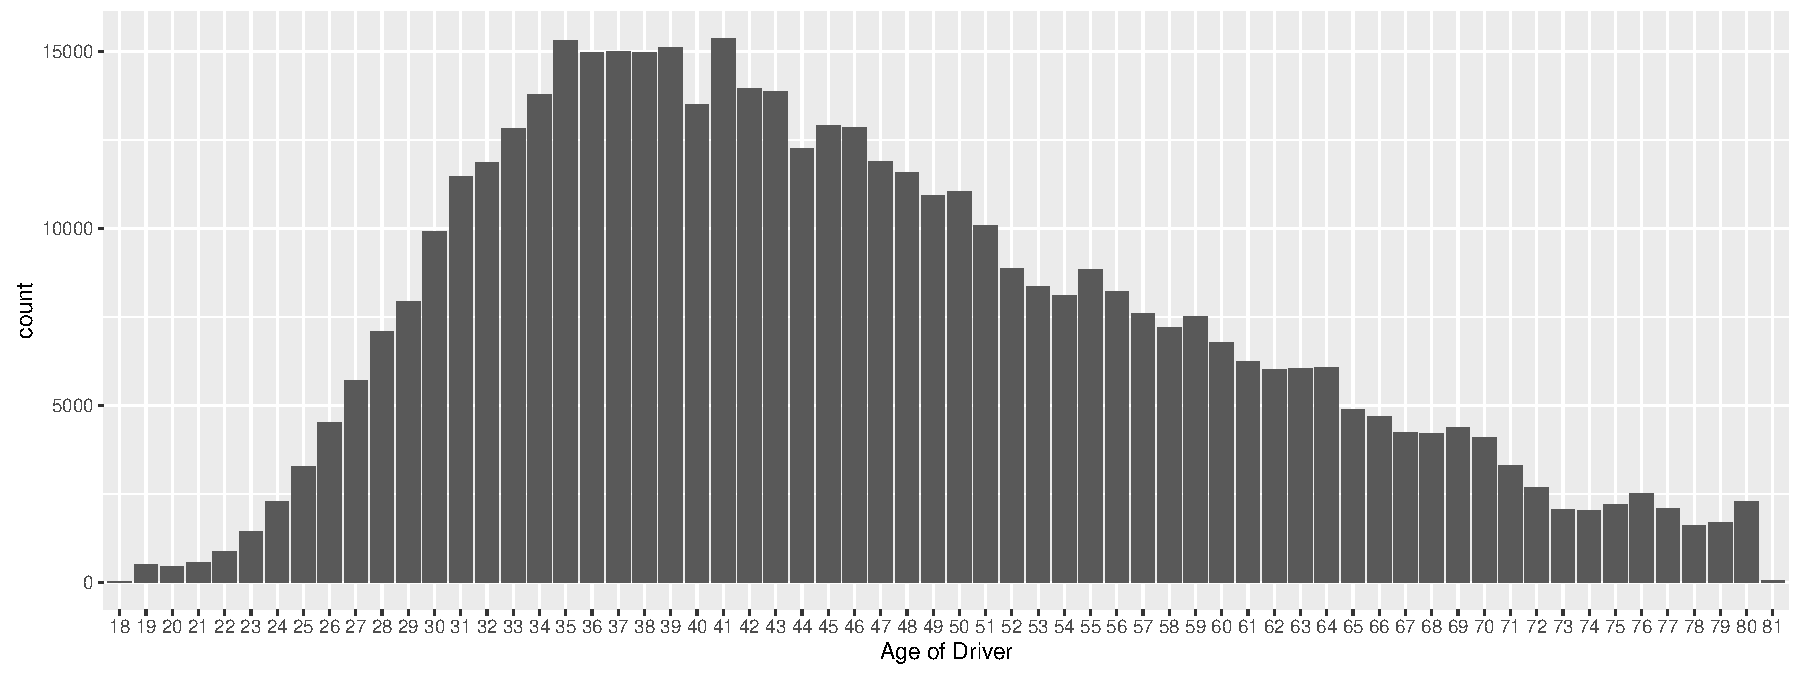
\includegraphics{variables_description_files/figure-latex/age_driver_dist_bar-1.pdf}

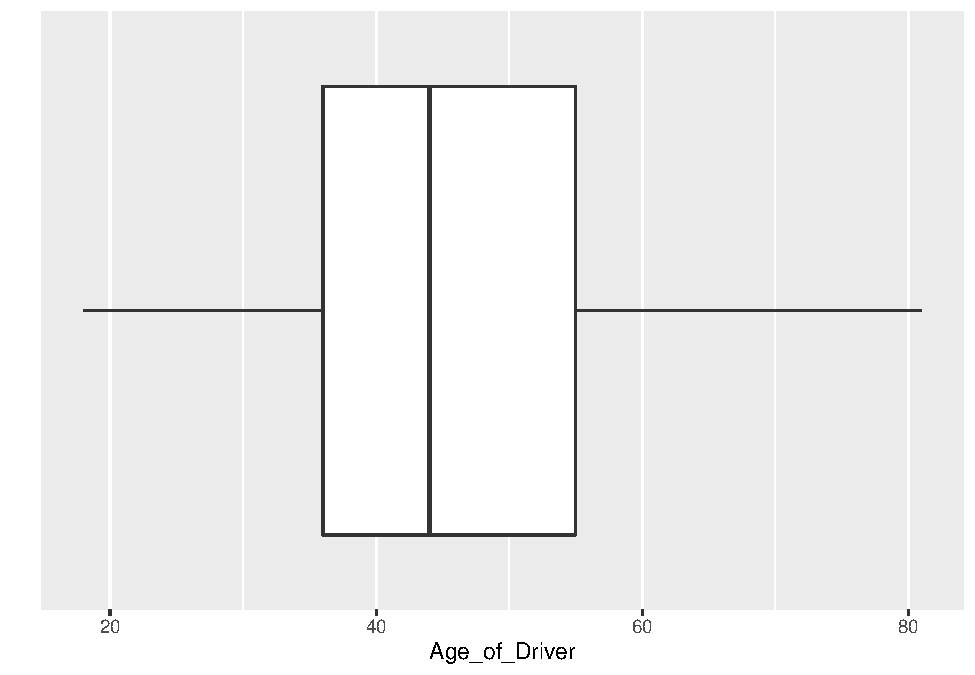
\includegraphics{variables_description_files/figure-latex/age_driver_dist_boxplot-1.pdf}

We can also split the histogram of age by the two possible policy
lengths (6 and 12)

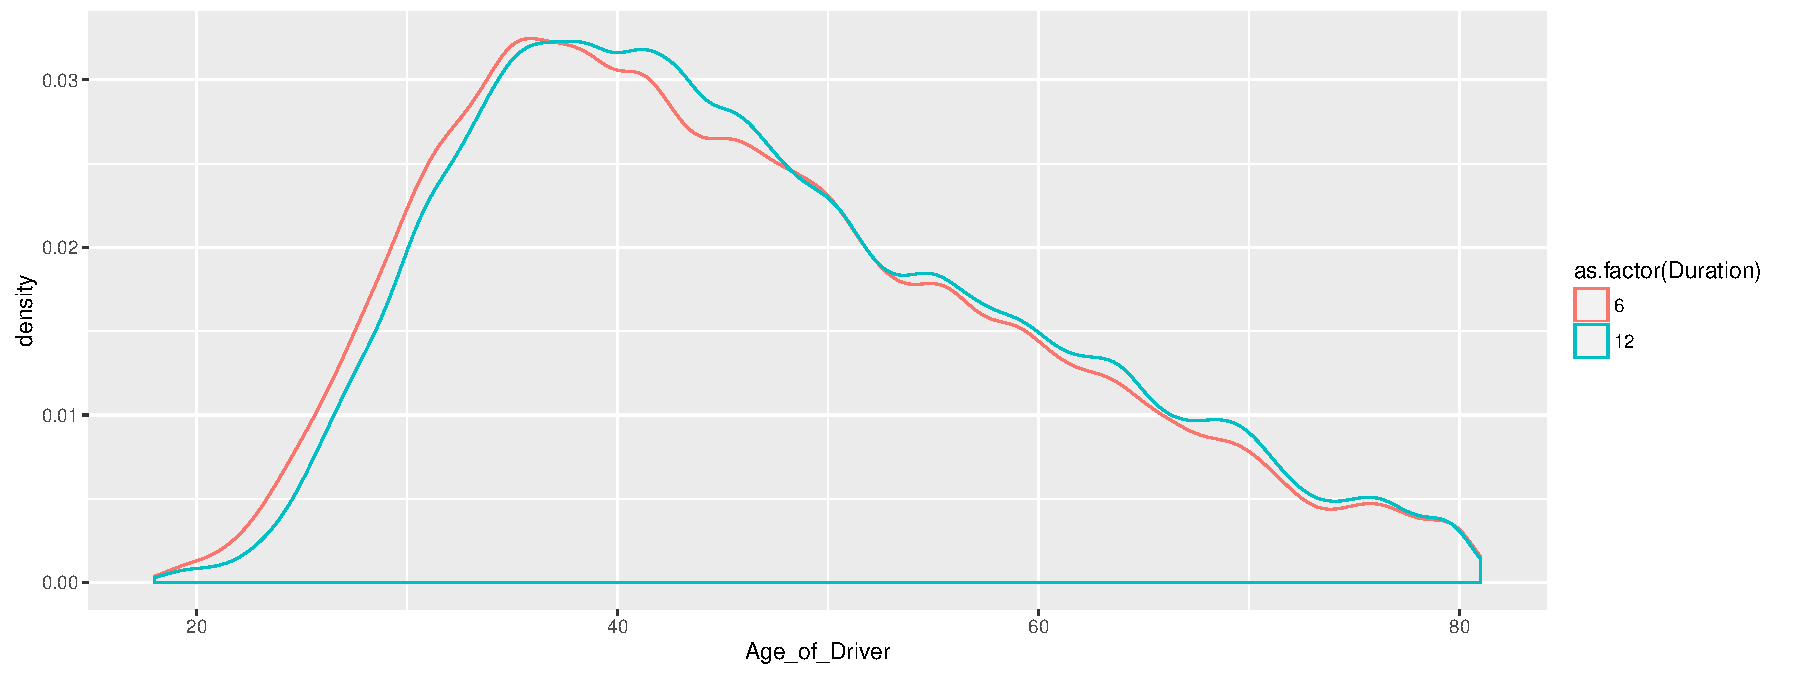
\includegraphics{variables_description_files/figure-latex/age_driver_dist_by_policy-1.pdf}

Proportion of under 26s that take on policies

\begin{verbatim}
## .
##         6        12 
## 0.6066914 0.3933086
\end{verbatim}

Proportion of over 70's that take out policies

\begin{verbatim}
## .
##         6        12 
## 0.4665278 0.5334722
\end{verbatim}

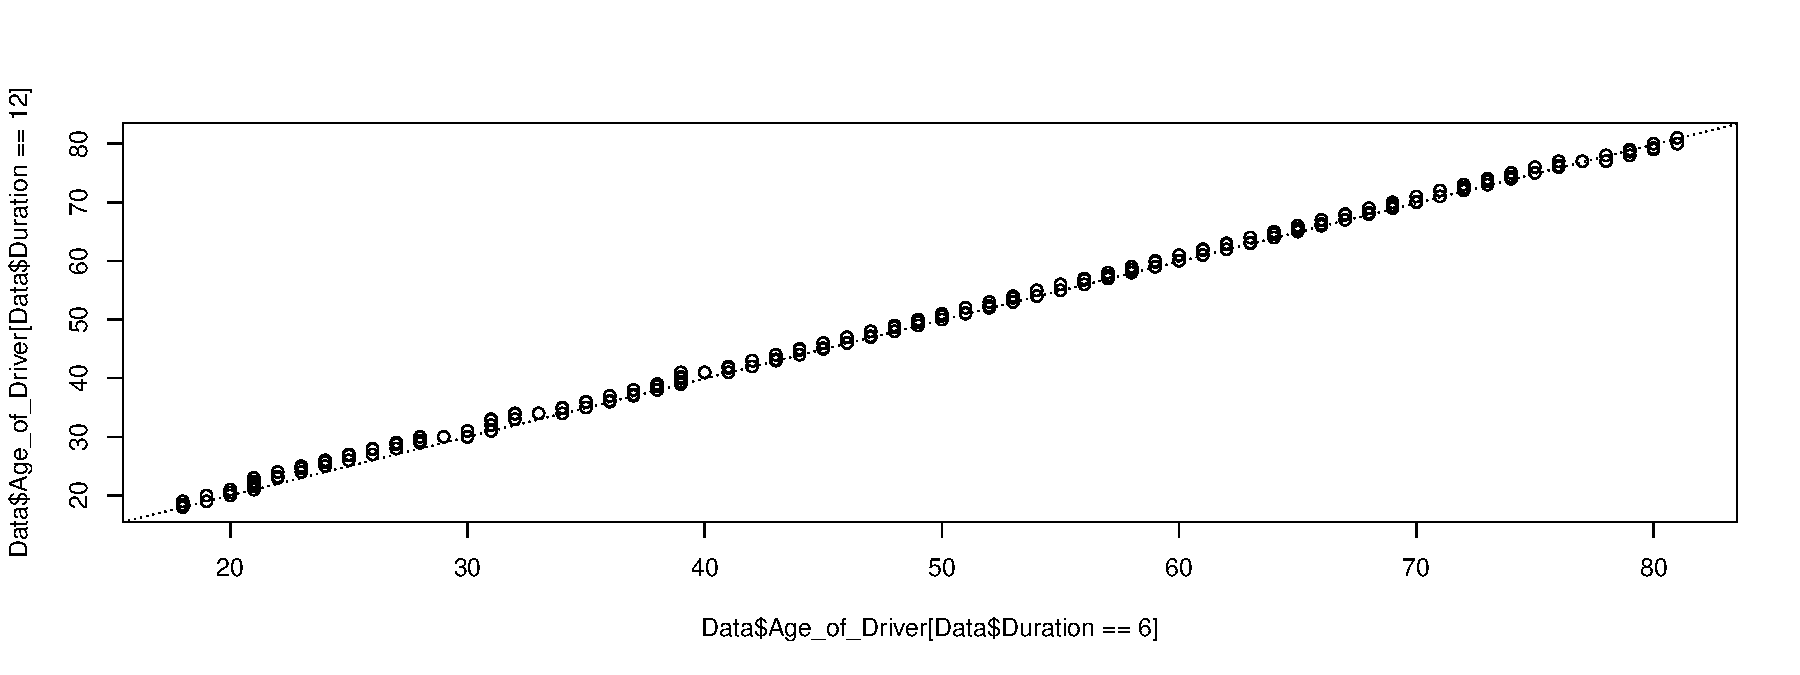
\includegraphics{variables_description_files/figure-latex/qqplot_age_policy-1.pdf}

\subsubsection{Age of Car}\label{age-of-car}

Car age distribution is shown below ranging from 0 to 31 years.

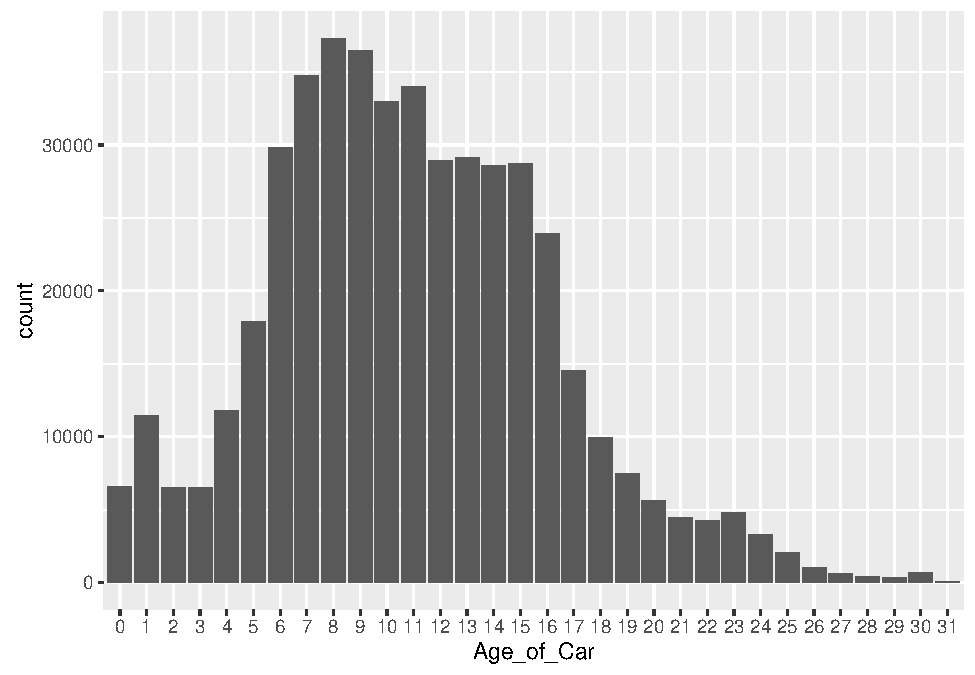
\includegraphics{variables_description_files/figure-latex/age_car_dist_bar-1.pdf}

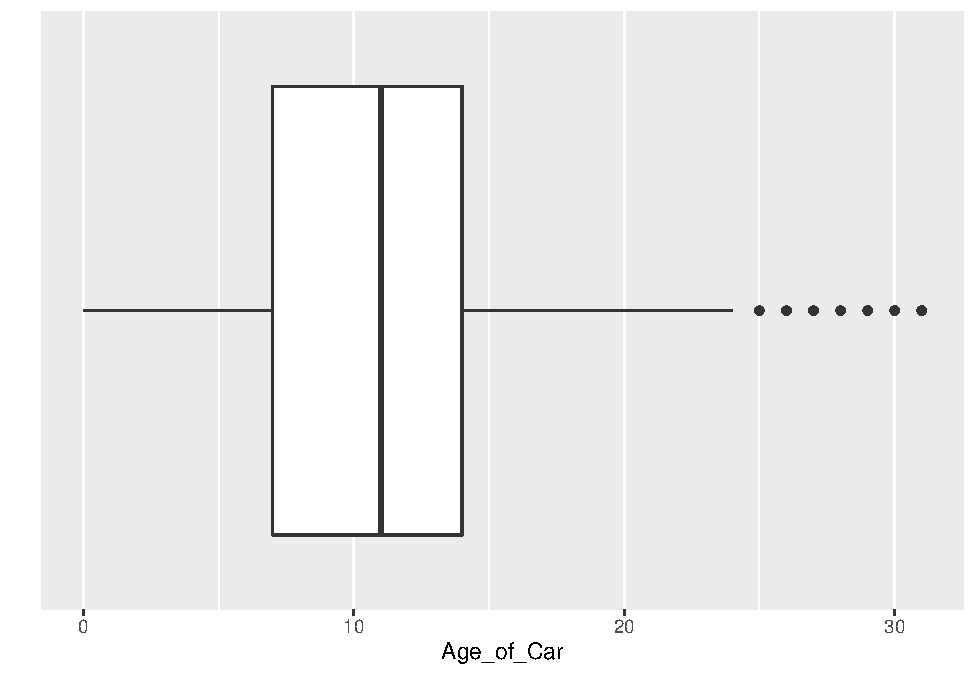
\includegraphics{variables_description_files/figure-latex/age_car_dist_boxplot-1.pdf}

\subsubsection{Expected Value of Car}\label{expected-value-of-car}

\begin{itemize}
\tightlist
\item
  There are a small number of extremely high valued cars
\item
  171 cars are valued above £50,000 - maxing out at £99,999.
\item
  What would be a sensible distance metric for dealing with the car
  values?
\end{itemize}

\begin{verbatim}
##    Min. 1st Qu.  Median    Mean 3rd Qu.    Max. 
##    1000    2000    4000    5320    7000  100000
\end{verbatim}

There are a number of expensive cars in this set making it difficult to
see the data clearly. This histogram is only for cars valued \textless{}
£40,000.

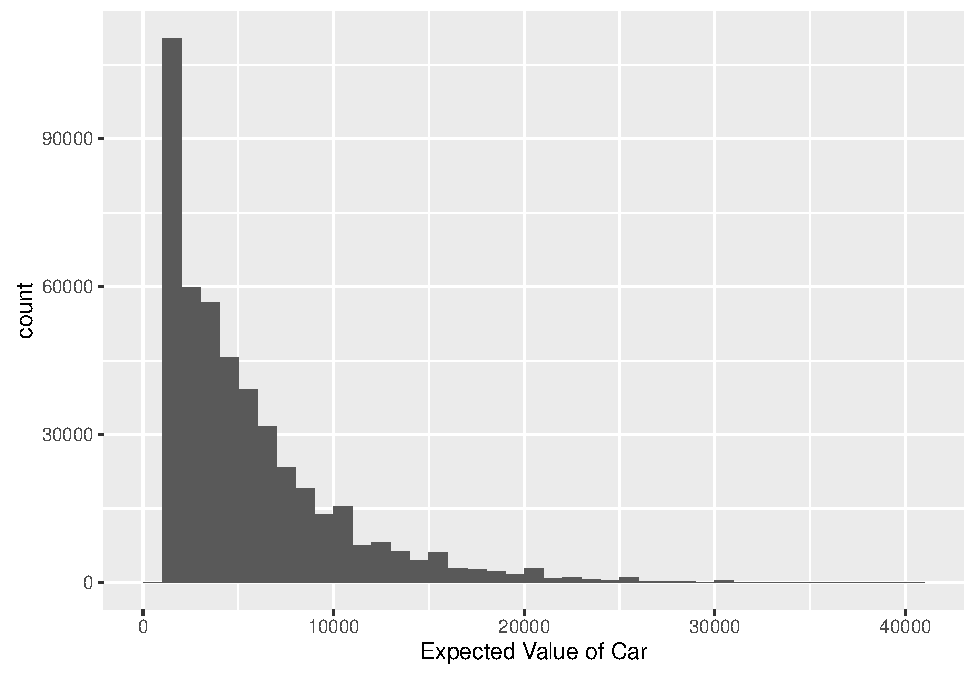
\includegraphics{variables_description_files/figure-latex/car_value_trunc_hist-1.pdf}

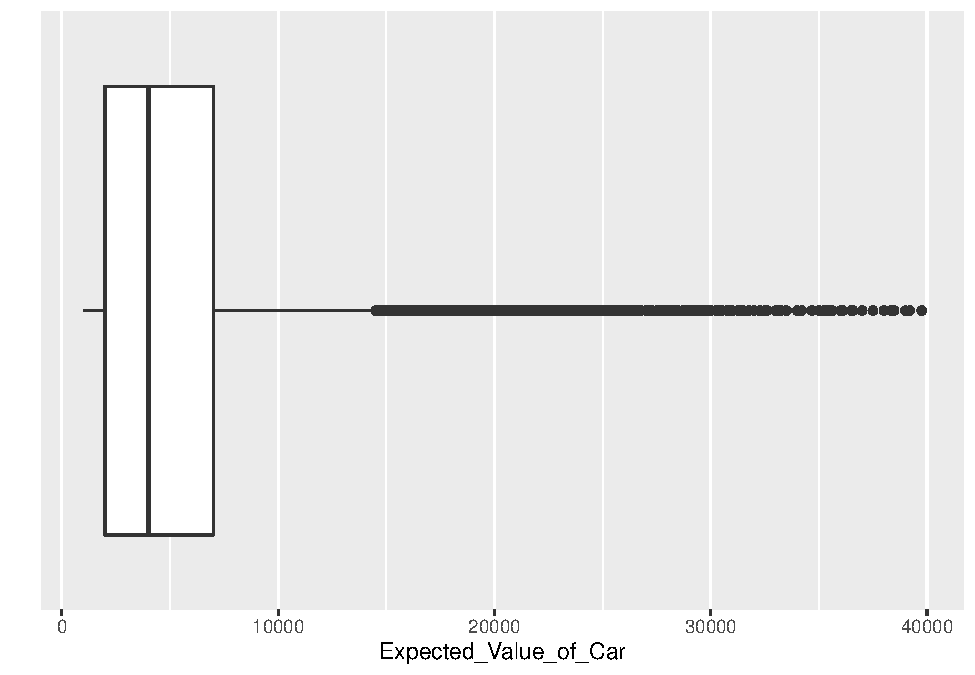
\includegraphics{variables_description_files/figure-latex/car_value_trunc_boxplot-1.pdf}

\subsubsection{Engine size (CC)}\label{engine-size-cc}

\begin{itemize}
\tightlist
\item
  Most cars have 1 - 2.5L engine
\item
  Some as low as 0.1L?
\item
  4000 cars with over 2.5L
\item
  Think about sensible distance metric
\end{itemize}

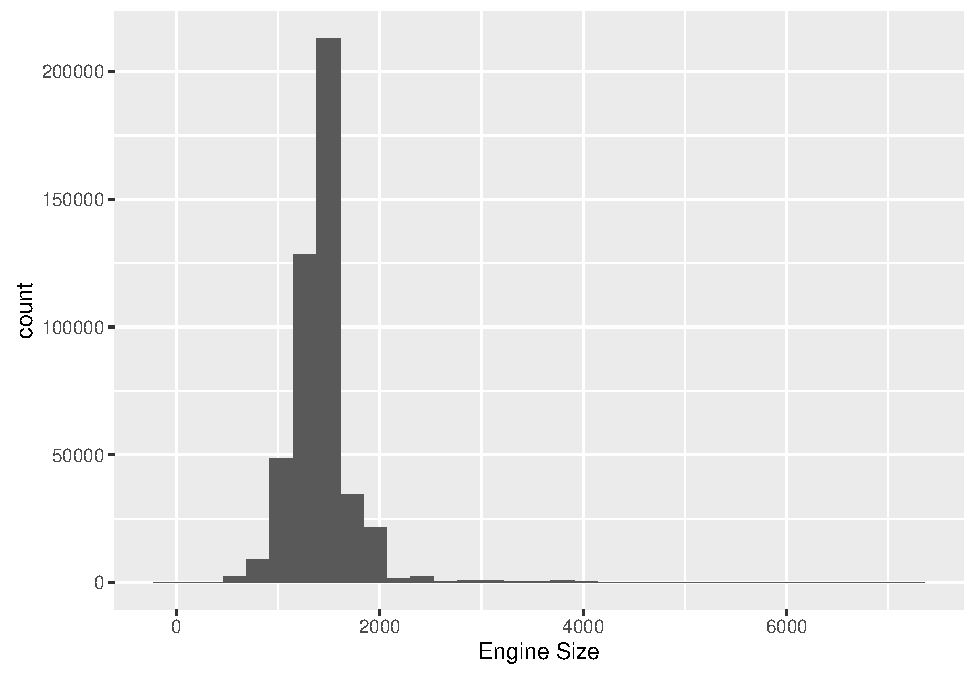
\includegraphics{variables_description_files/figure-latex/cc_hist-1.pdf}

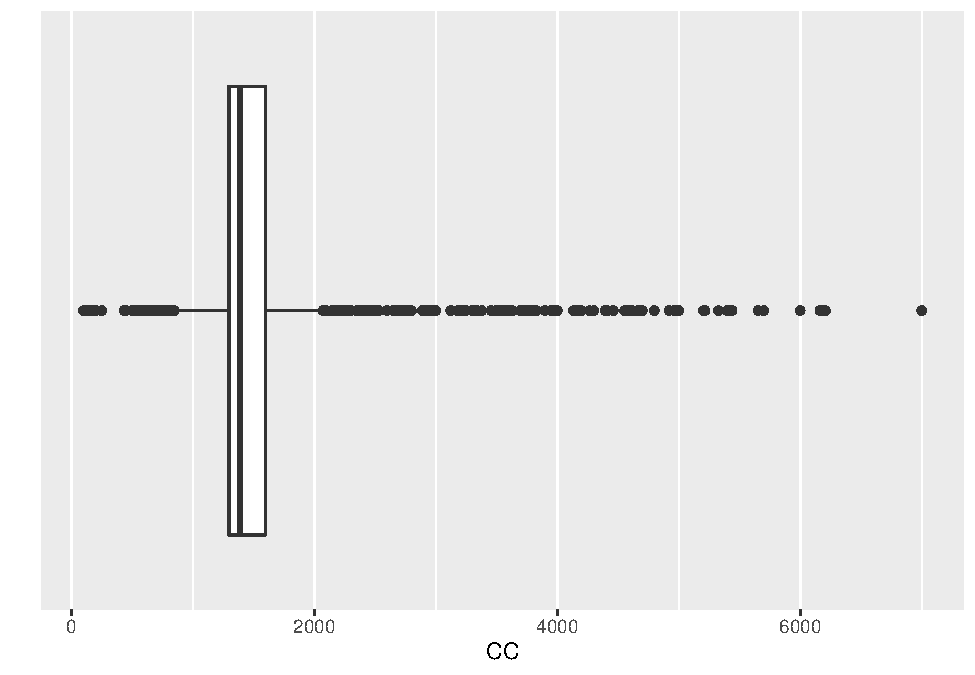
\includegraphics{variables_description_files/figure-latex/cc_boxplot-1.pdf}

\subsubsection{Duration}\label{duration}

Binary factor either 6 or 12. Assume this is duration of policy in
months.

\begin{itemize}
\tightlist
\item
  224578 6 months policies
\item
  240537 12 month policies
\end{itemize}

\subsubsection{Values A, B and C}\label{values-a-b-and-c}

\begin{itemize}
\tightlist
\item
  I assume these are policy quotes for different schemes?
\item
  Value A \textless{} Value B \textless{} Value C is always true for
  each row
\item
  Therefore I assume that Value A is a basic policy and Value C is a
  premium policy
\item
  We would expect 6 month policies to be cheaper than 12 month policies
\end{itemize}

We can look at simple summaries of the three policies offered

\begin{verbatim}
##    Min. 1st Qu.  Median    Mean 3rd Qu.    Max. 
##    44.0   117.0   167.0   173.7   222.0   701.0
\end{verbatim}

\begin{verbatim}
##    Min. 1st Qu.  Median    Mean 3rd Qu.    Max. 
##    56.0   129.0   188.0   192.3   246.0   716.0
\end{verbatim}

\begin{verbatim}
##    Min. 1st Qu.  Median    Mean 3rd Qu.    Max. 
##    75.0   155.0   225.0   231.3   297.0  1667.0
\end{verbatim}

The values A,B,C have skewness of 0.6571885 0.5329351 and 0.6267024
respectively.

We can also look at a plot of the sorted Values to see how they
interact.

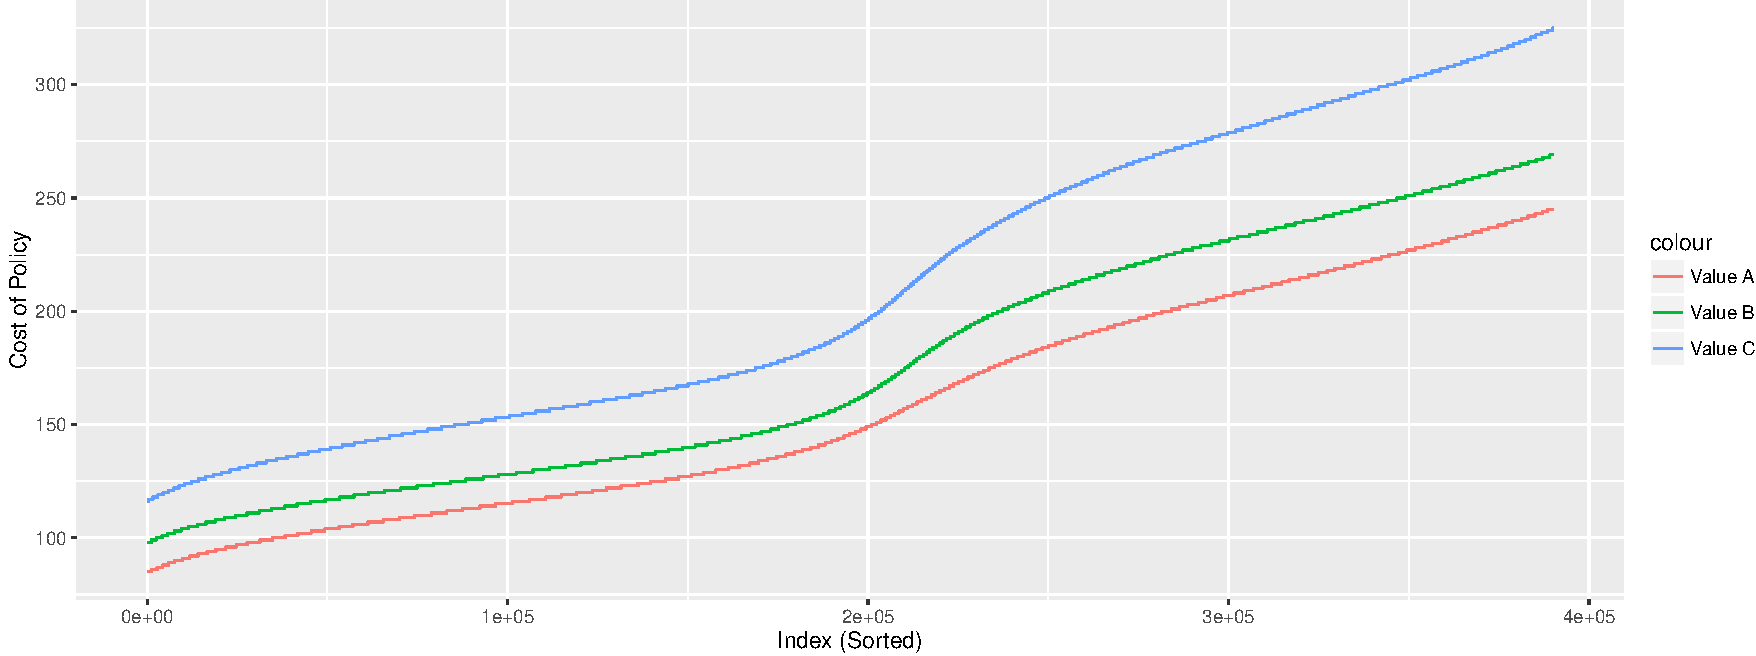
\includegraphics{variables_description_files/figure-latex/values_sorted-1.pdf}
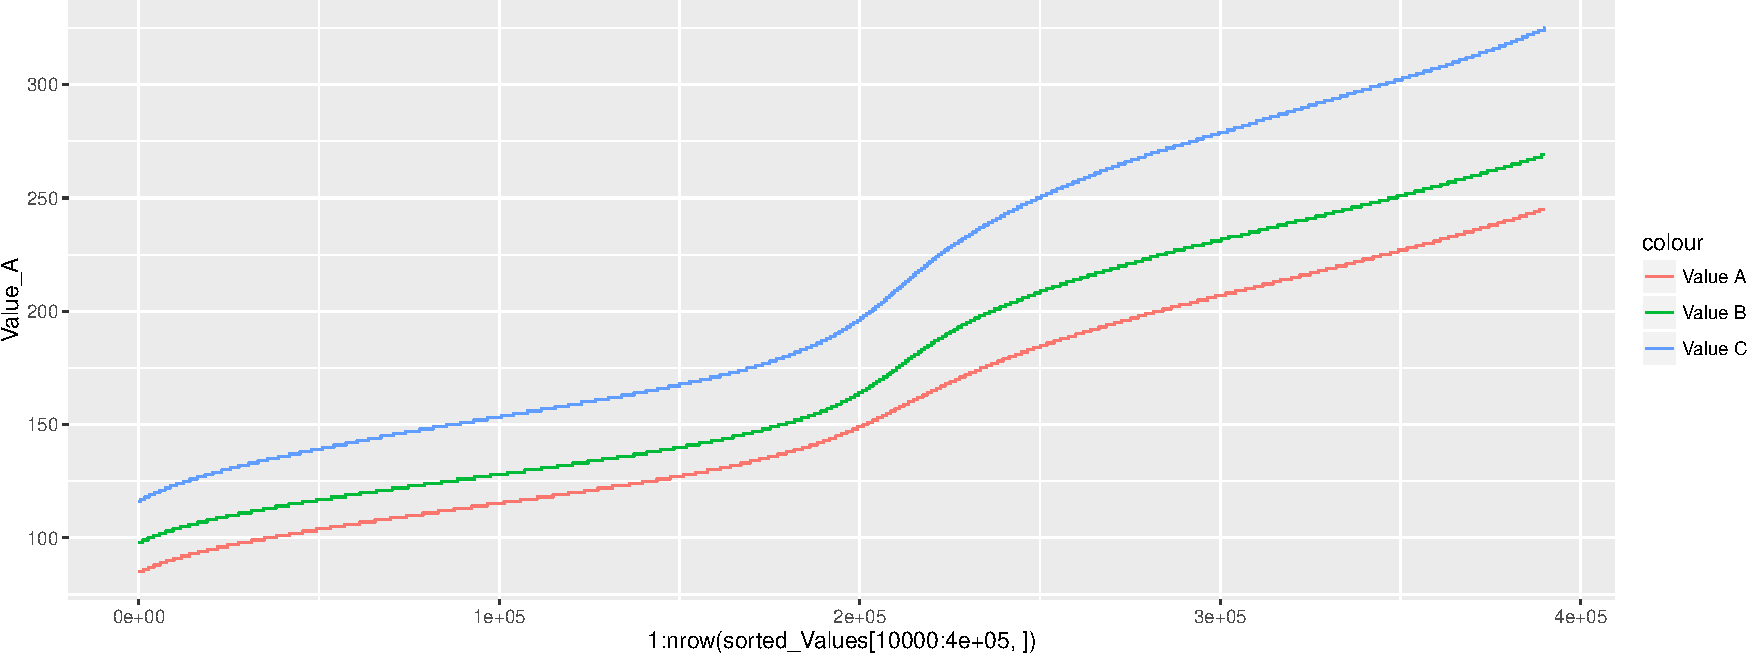
\includegraphics{variables_description_files/figure-latex/values_sorted-2.pdf}

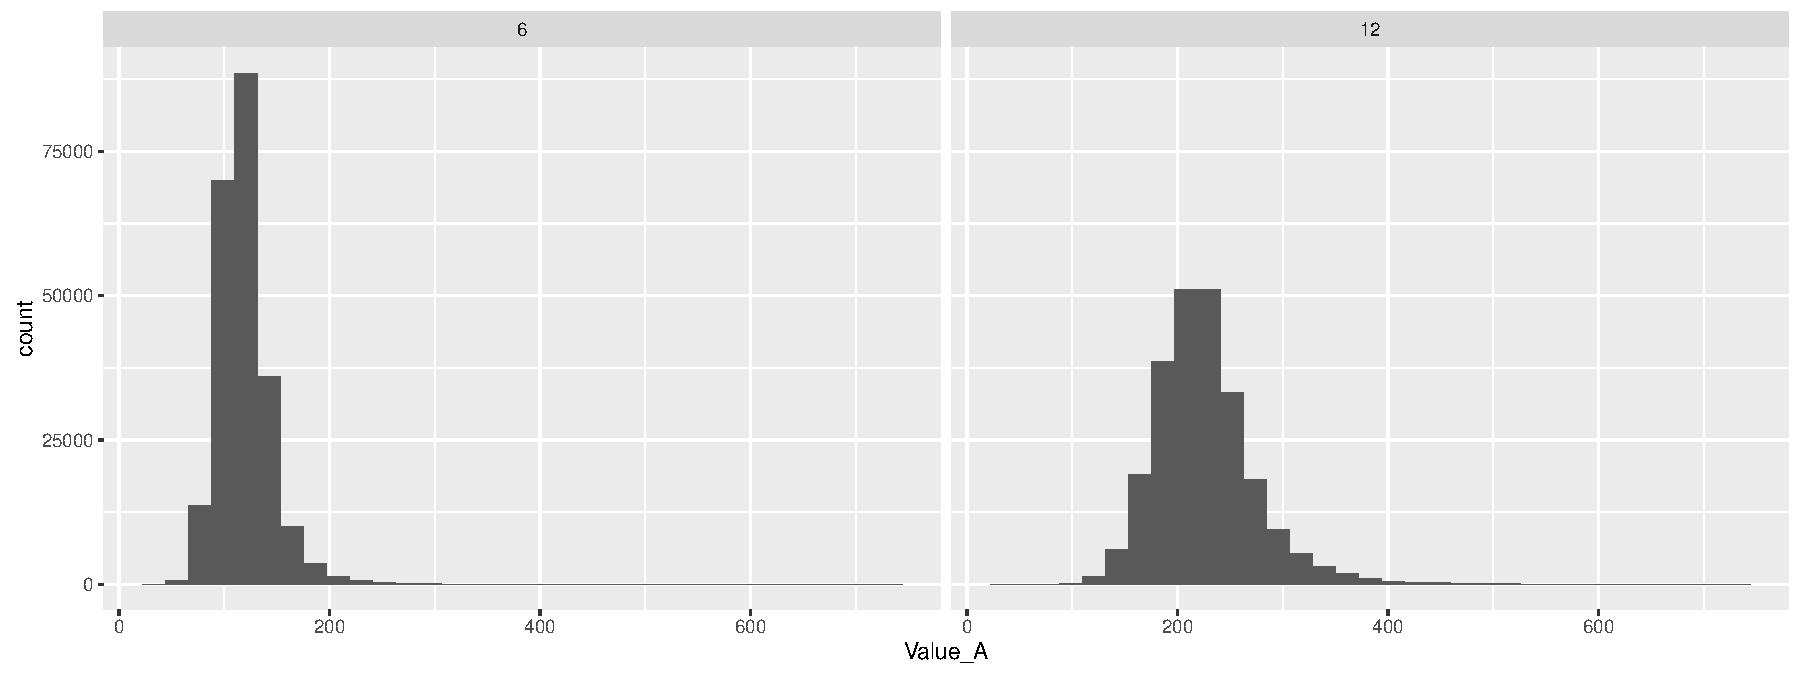
\includegraphics{variables_description_files/figure-latex/values_boxplots-1.pdf}
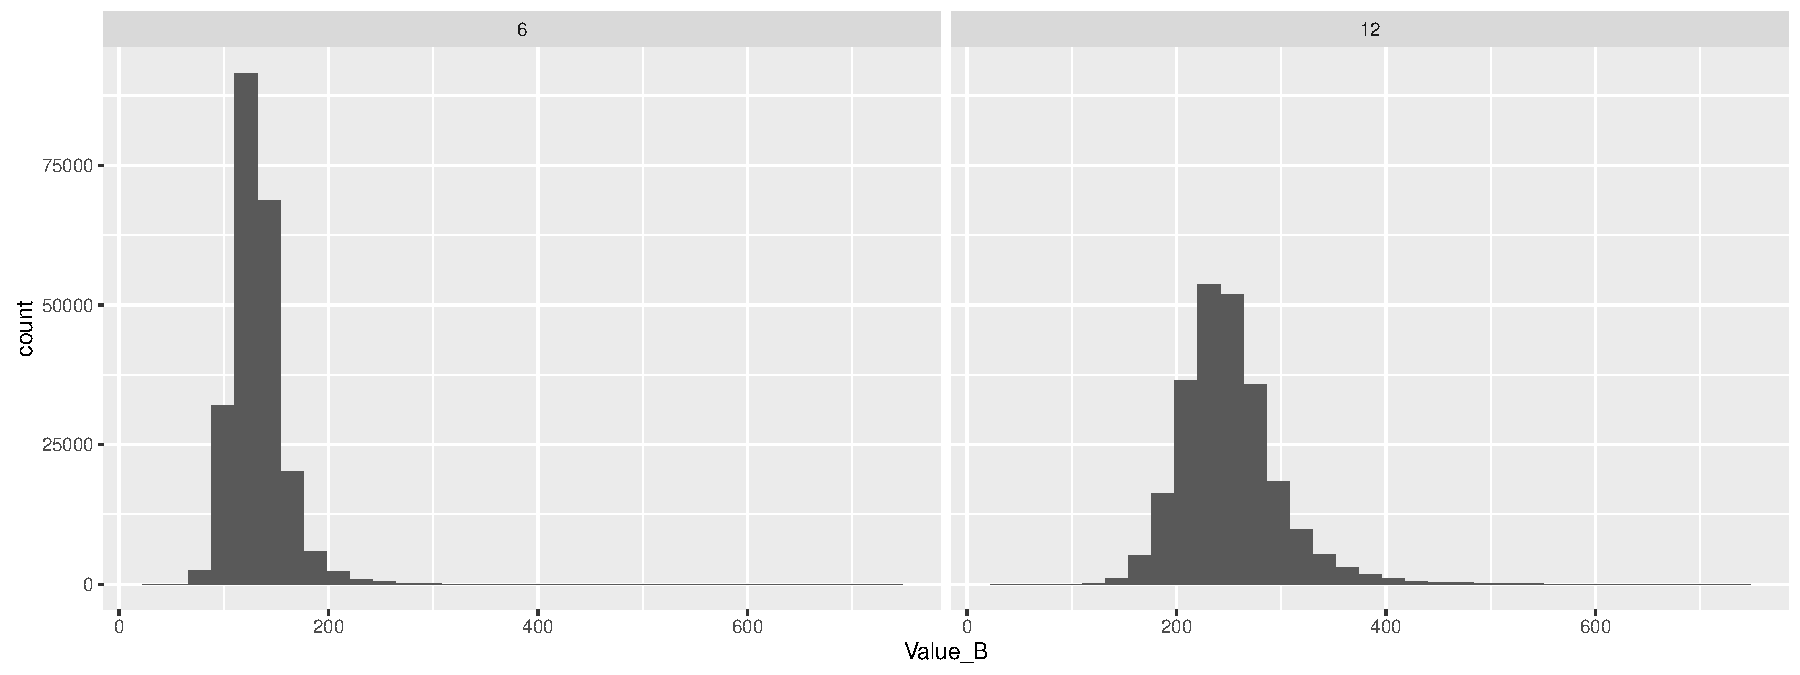
\includegraphics{variables_description_files/figure-latex/values_boxplots-2.pdf}
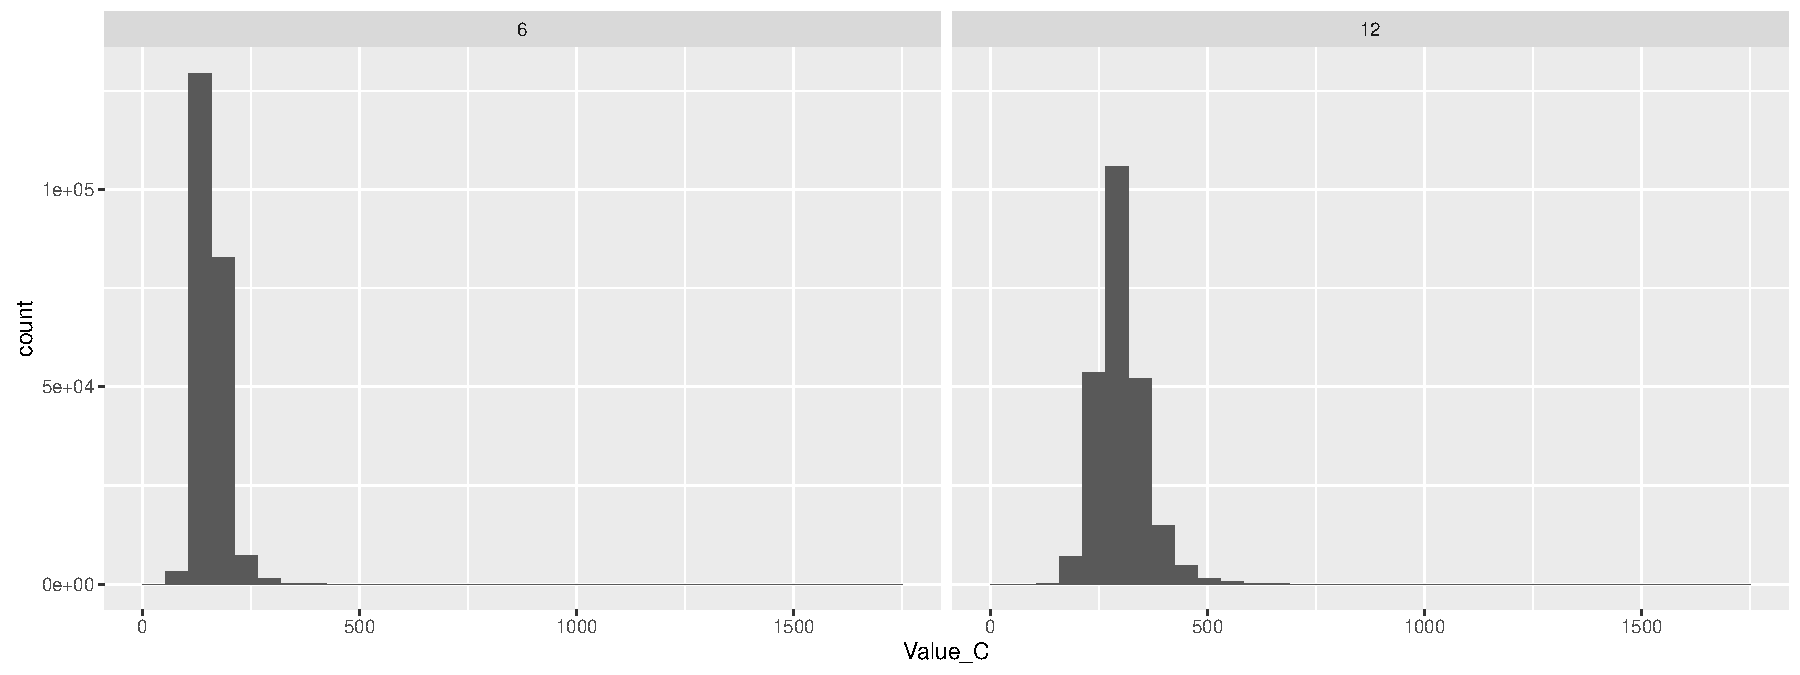
\includegraphics{variables_description_files/figure-latex/values_boxplots-3.pdf}


\end{document}
